Please describe the achieved outcomes of the project.
If possible, please provide figures showing the described outcomes.
Please confront them with the objectives of the project.
This part should be between 2000 and 10,000 characters long.
Please use Times New Roman font, 12 pts, 1.5 spacing.
Full description of solutions that were worked out and project outcomes, if any, should be presented in annexes.
\begin{figure}[H]
    \centering
    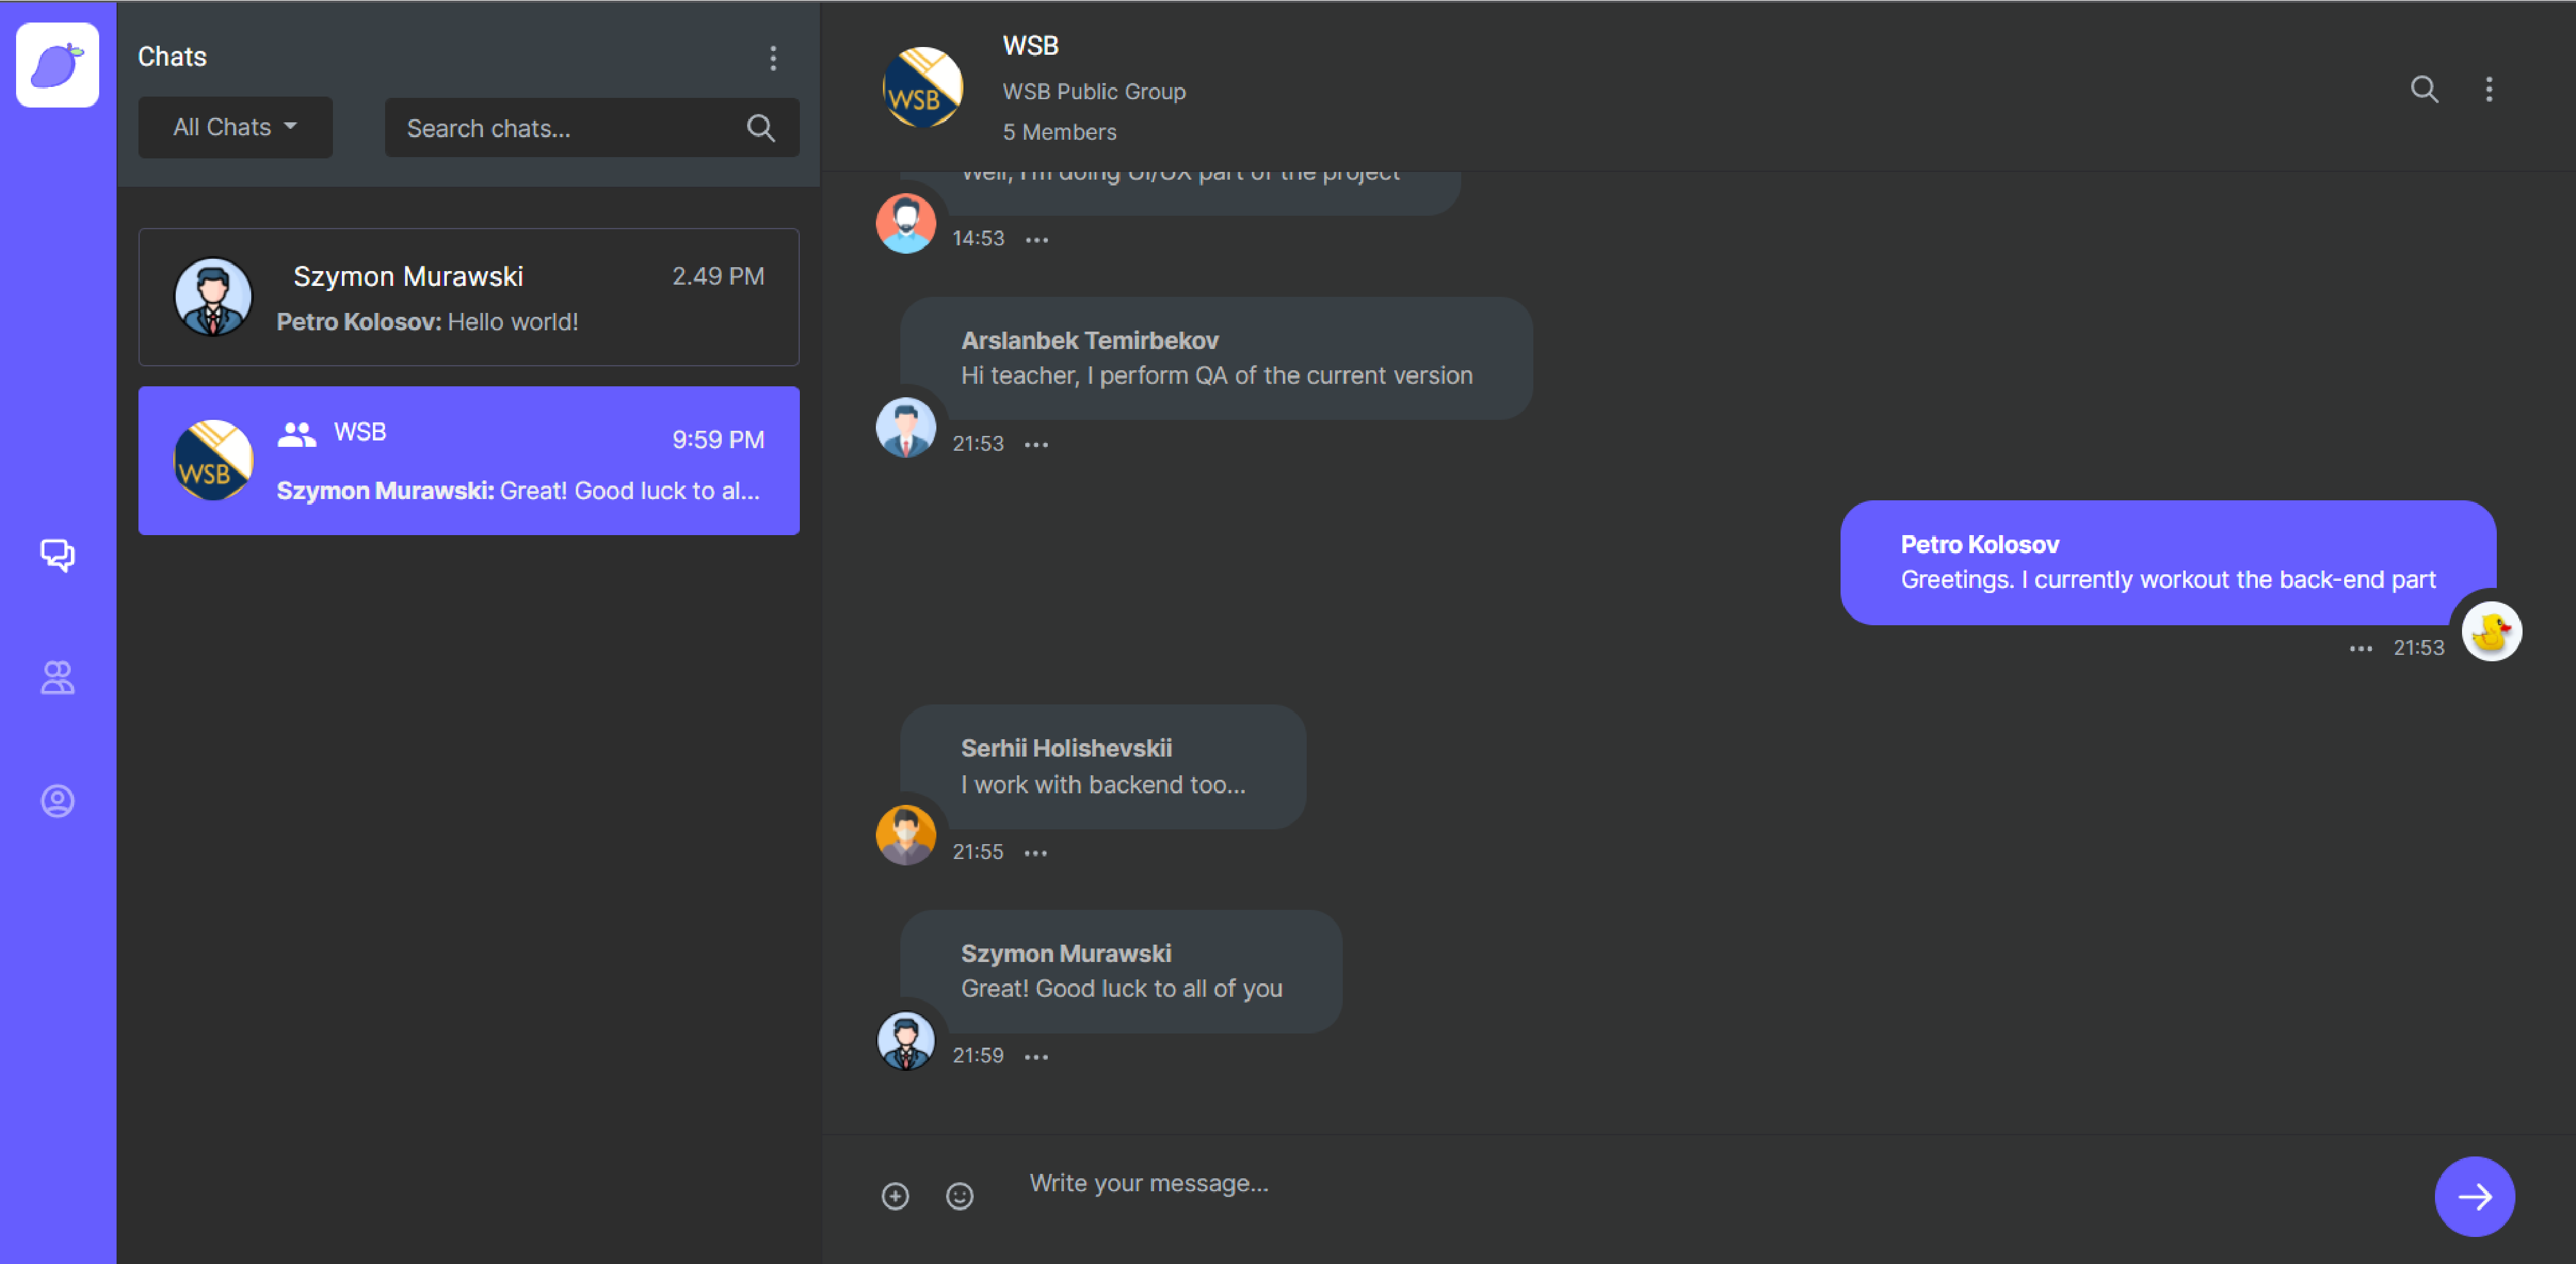
\includegraphics[width=1\textwidth]{Pictures/Messenger-1}
    \caption{Secret chat encryption concept diagram. Source: }\label{fig:figure5}
\end{figure}

\begin{enumerate}
    \item In the screenshot 2.9, on the left, there is a list of the user's chats.
    \item In the screenshot 2.9, on the top left, there is a field for text input, entering a certain text,
    and clicking on the enter or on the icon with a magnifying glass the user can find the chat he is interested in,
    containing the entered text in its name.
    \item In the screenshot 2.9, on the top left, there is an icon with three dots, by clicking on which a button will appear to create a chat,
    by clicking on it, you can go to the creation of a chat.
    \item In the screenshot 2.9, on the top left there is a button, by clicking on which a drop-down list appears,
    by clicking on a specific one, you can choose to filter the displayed chats.
    \item In the screenshot 2.9, on the right, there is a magnifying glass icon, by clicking on which you can search by messages in a particular chat.
    \item In the screenshot 2.9, on the right, there is an icon with three dots, by clicking on which 2 buttons will appear,
    by clicking on the first user can (un)archive the chat, by clicking on the second user can leave the chat.
    \item In the screenshot 2.9, at the bottom there is a field for entering text, entering text into it,
    and clicking on the enter or on the arrow icon at the bottom right,the user can send a message to a specific chat.
    \item In the screenshot 2.9, below, to the left of the text message input field, there is an icon with a smiley by clicking on it,
    and by clicking on a specific emoji, the user can add it to his text message.
    \item In the screenshot 2.9, below, to the left of the emoticon icon, there is an icon with a plus by clicking on it, then selecting the file,
    the user can send the selected file to a specific chat by clicking on the send button.
\end{enumerate}

\begin{figure}[H]
    \centering
    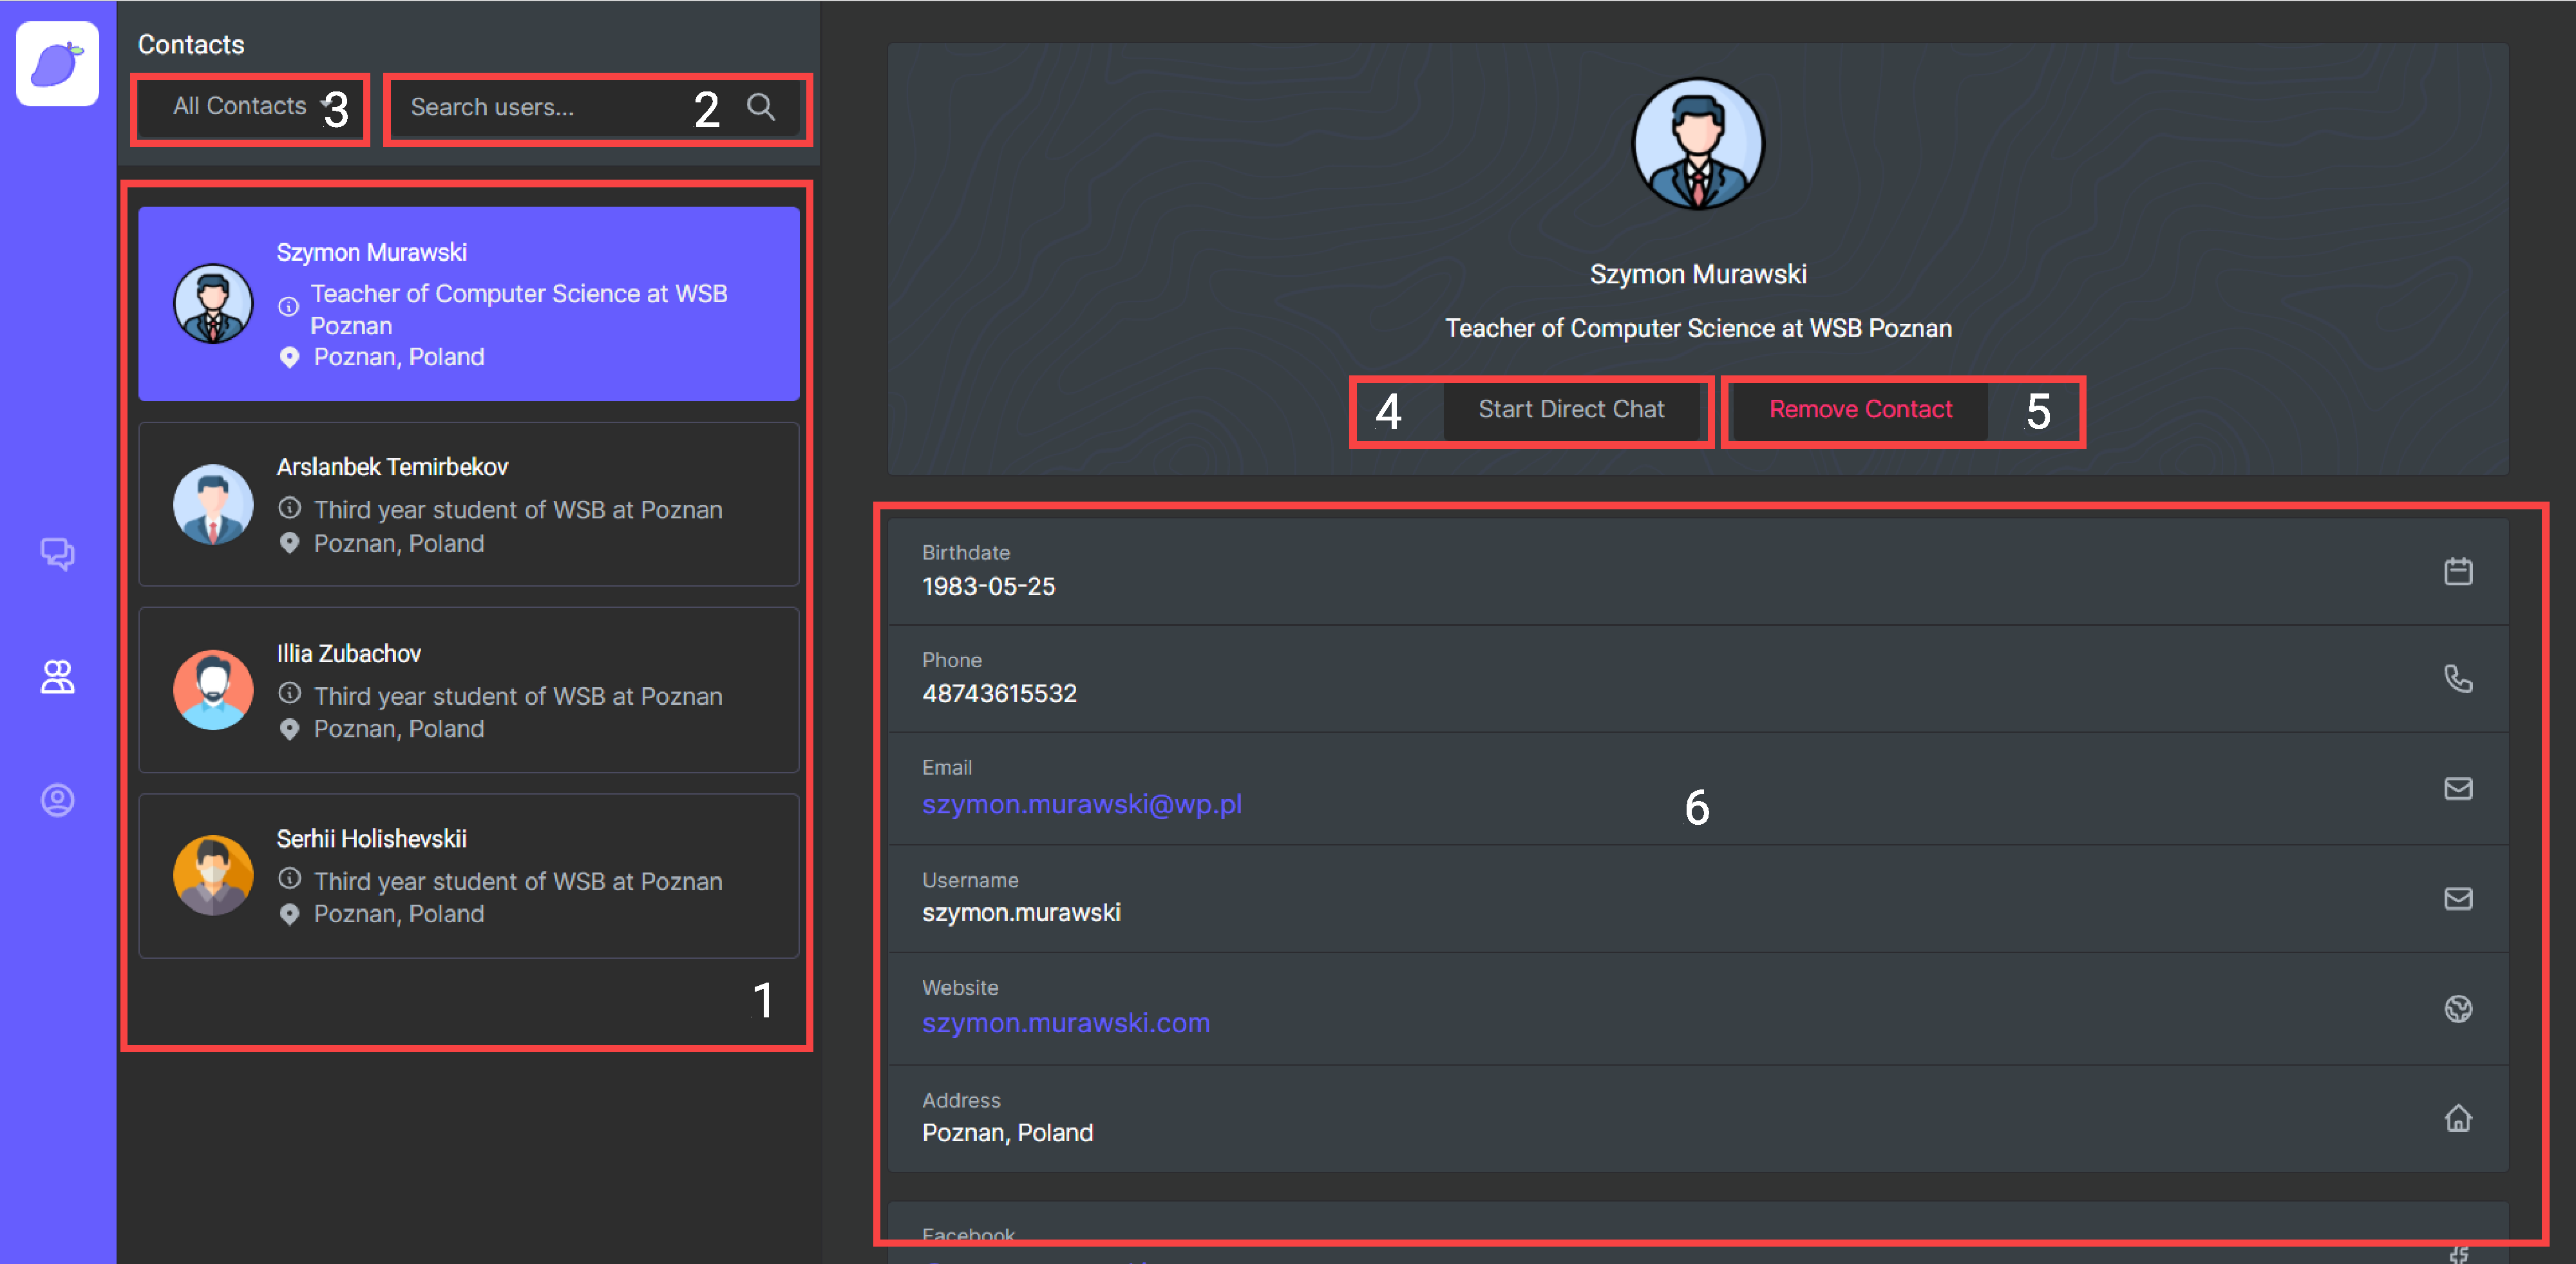
\includegraphics[width=1\textwidth]{Pictures/Messenger-2}
    \caption{Secret chat encryption concept diagram. Source: }\label{fig:figure10}
\end{figure}
\begin{enumerate}
    \item In the screenshot 2.10, on the left there is a list of user contacts, by clicking on a specific one,
    information about the contact will be displayed on the right and two buttons,
    the first allows you to start a chat with a specific user, and the second button removes the user from the contact list.
    \item In the screenshot 2.10, on the left, there is a field for entering text, entering certain text, and clicking on the enter or on the magnifying glass,
    will display users who have a phone number/email/display name contains the entered text,
    by selecting one of the displayed, you can add it to your contacts, start with a chat and get information about it.
    \item In the screenshot 2.10, on the left, there is a button for filtering contacts, by clicking on it, a drop-down list appears,
    in which you can select a filtering method: "All contacts", "Search results".
\end{enumerate}

\begin{figure}[H]
    \centering
    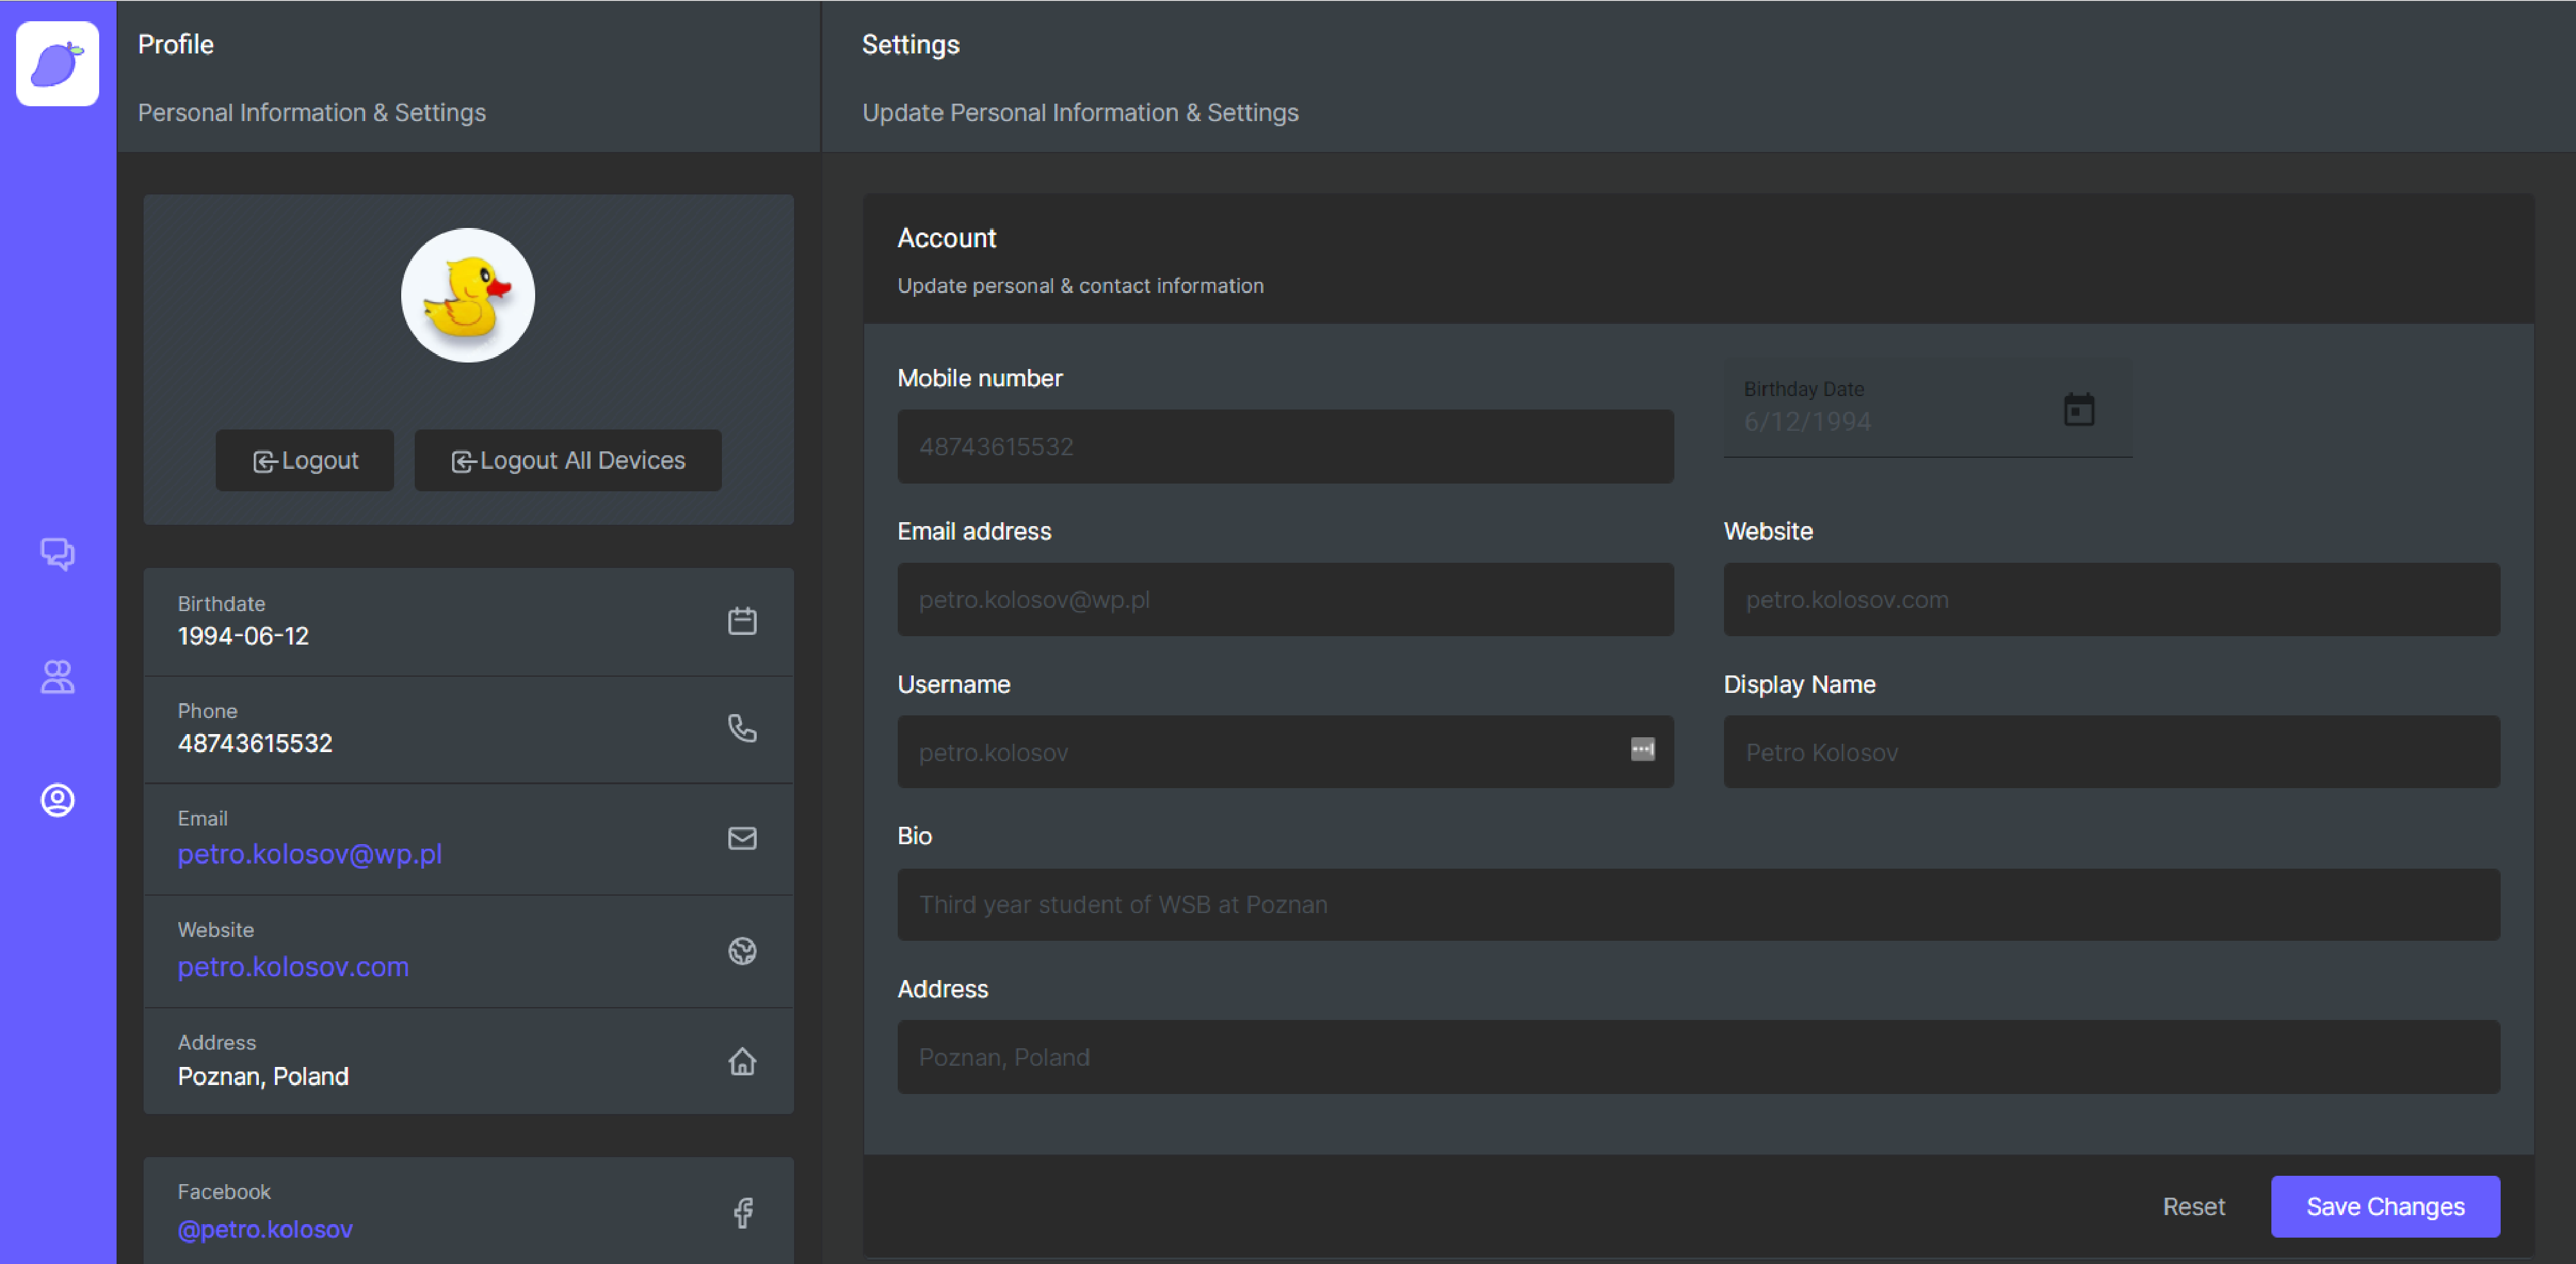
\includegraphics[width=1\textwidth]{Pictures/Messenger-3}
    \caption{Secret chat encryption concept diagram. Source: }\label{fig:figure11}
\end{figure}
\begin{enumerate}
    \item In the screenshot 2.11, on the left, there is the user's current information, his avatar, and two button buttons,
    the first one logs out of the account on this device,
    and the second button logs out the account from all devices.
    \item In the screenshot 2.11, in the center, displayed the user settings, there are fields for updating personal data,
    updates of links to social networks.
\end{enumerate}